\textbf{Note:} \textit{The following contents are not part of the Probability Theory course at Imperial College London from 2021 onwards. We are including the materials for completion, and to provide readers necessary backgrounds for further studies in probability theory and stochastic processes.}

\section{Martingales*}
We almost have enough tools to discuss the notion of martingales $(\xi_n)_{n\geq 0}$, which is one of the most fundamental classes of stochastic processes. It captures the uncertainty of random walks, that one cannot guess the general direction of the movement of the walking object by looking at the path history. Therefore, this notion of stochastic processes is applied extensively in many areas, including mathematical finances.

\begin{remark}
We will usually assume that the stochastic process $(\xi_t)$ to be indexed by $t \in \N$ or $t \in [0,\infty)$. If $t \in \N$ we call the stochastic process \textit{discrete-time}, and if $t \in [0,\infty)$ we call the stochastic process \textit{continuous-time}. Results about discrete-time stochastic processes can be extended to continuous-time stochastic processes easily most of the time, but not always. We will therefore focus on \textit{discrete-time} processes in this chapter, and provide a sketch on how the notion can be generalised to continuous times.
\end{remark}

\subsection{Filtration}
Before delving into the details, one needs to formalise the notion of "path history". This is captured by a 

\begin{definition}[Filtration]
A filtration of a probability space $(\Omega,\F,\p)$ is an increasing sequence of sub-$\sigma$-algebra $(\F_t)_{t\geq 0}$ of a  such that $\F_s \subseteq \F_t$ whenever $s \subseteq t$.
\end{definition}

The sequence can be countable or uncountable, depending on whether we want to talk about discrete or continuous-time stochastic processes. We say that 

\begin{definition}[Adapted Processes]
a stochastic processes $(\xi_t)_{t\geq 0}$ is \textbf{adapted} to this sequence of sub-$\sigma$-algebra if $\xi_t$ is $\F_t$-measurable, i.e. $\sigma(\xi)_t \subseteq \F_t$.
\end{definition}

In such case, we also see that $\xi_s$ are also $\F_t$-measurable whenever $s \leq t$, so one may use sets in $\F_t$ to describe any events relating to the past $(\xi_s)_{0\leq s < t}$. Therefore, for any $t$, $\F_t$ captures the path history during the time period of $s < t$. We will impose this assumption for any stochastic processes we consider.

\begin{example}[Natural Filtration]
Recall that we can always enlarge a collection of subsets of $\Omega$ so that it becomes a $\sigma$-algebra. With this in mind, given a stochastic process $(\xi)_{t\geq 0}$ of $(\Omega,\F,\p)$, one may construct the $\sigma$-algebra
\begin{equation}
    \F_t = \bigvee_{s \leq t} \sigma(\xi_s),
\end{equation}
which is the smallest $\sigma$-algebra containing $\sigma(\xi_s)$ for all $s<t$. The sequence $(\F_t)_{t\geq 0}$ is then a filtration, for which $(\xi_t)_{t\geq 0}$ is adapted to, and we call this the \textit{natural} filtration of $(\xi_t)_{t\geq 0}$. A discrete example has already been discussed in definition \ref{def:discrete_natural_filtration} when we define the tail $\sigma$-algebra for the Kolmogorov's 0-1 law.
\end{example}

We consider the example of tossing a coin. Recall that there are at least two ways to define this stochastic process. Let's say we define this as a sequence of random variables $(\xi_n)_{n\geq 1}$ on a common probability space $(\set{0,1}, 2^{\set{0,1}},\p)$ as in section 4.1. For this sequence of random variables to be adapted to a filtration $(\F_n)_{n\geq 1}$, the filtration must satisfy

\begin{itemize}
    \item $\F_1$ contains $\varnothing, \set{\xi_1 = 0}, \set{\xi_1 = 1}, \set{\xi_1 = 0} \cup \set{\xi_1 = 1} = \Omega$,
    \item $\F_2$ contains $\varnothing$, $\set{\xi_1 = 0, \xi_2 = 0}$, $\set{\xi_1 = 0, \xi_2 = 1}$, $\set{\xi_1 = 1, \xi_2 = 0}, \set{\xi_1 = 1, \xi_2 = 1}$, $\set{\xi_1 = 0}$, $\set{\xi_1 = 1}$, $\set{\xi_2 = 0}$, $\set{\xi_2 = 1}$, $\Omega$,
    \item so on and so forth.
\end{itemize}

The elements in $\F_n$ can be easily described. For instance, the set $\set{\xi_1 = 1, \xi_2 = 0, \xi_3 = 0}$ can be described as any sequences $\omega \in \set{0,1}^{\otimes \N}$ that starts with $1, 0, 0, ...$ The sets are, however, difficult to be visualised.

\begin{exercise}
For easier figure representation, one might also consider the second setup of tossing a coin using Rademacher functions (see subsubsection 4.1.1). Again, give a representation of what the elements in $\F_n$ represent, and draw them on a real line. 
\end{exercise}

% an inaccurate representation 

\subsection{Martingales: definitions and examples}
With the notion of filtration and adapted processes, one can easily represent the notion of martingales using conditional expectation. Here we also define two more notions of stochastic processes: super- and sub-martingales.

\begin{definition}[Super-/Sub-martingales]
Consider the stochastic process $(\xi_t)_{t\geq 0}$ adapted to the filtration $(\F_t)_{t\geq 0}$, \textbf{so that $\forall t, \E|\xi_t|<\infty$}, then it is a 
\begin{itemize}
    \item $(\F_n)$-\textbf{sub-martingale} if $\forall s \leq t, \xi_s \leq \E[\xi_{t} \,|\, \F_s]$, 
    \item $(\F_n)$-\textbf{super-martingale} if $\forall s \leq t, \xi_s \geq \E[\xi_{t} \,|\, \F_s]$,
    \item $(\F_n)$-\textbf{martingale} if $\forall s \leq t, \xi_s = \E[\xi_{t} \,|\, \F_s]$, i.e. the stochastic process is both a $(\F_n)$-sub-martingale and $(\F_n)$-super-martingale.
\end{itemize}
\end{definition}

We make a few quick observations before delving into the examples:
\begin{remark} \label{rmk:martingale_first_observations}
\begin{enumerate}
    \item[]
    \item As a reminder, we only need the (in-)equalities above holds \textit{almost surely}, as the conditional expectations above are defined almost surely anyway.
    \item The above notions all depend on the filtration we use, and unless otherwise specified we will assume using natural filtration when discussing martingales in real-life applications.
    \item It is quite clear that if the stochastic process $(\xi_t)_{t\geq 0}$ is a sub-martingale, then the stochastic process $(-\xi_t)_{t\geq 0}$ is a super-martingale.
    \item For the case when the stochastic process $(\xi_t)_{t\geq 0}$ and filtration $(\F_t)_{t\geq 0}$ are discrete-time, i.e. indexed by $t \in \N$ (for which we replace the indices $t$ by $n$), one can show that it is a sub-martingale by comparing what's happened in the present and immediate future (or immediate past), i.e. showing $\xi_n \leq \E[\xi_{n+1} \,|\, \F_n]$ due to the tower law (see property \ref{prop:tower_property_general}). Analogous results hold for super-martingales and martingales as well.
    \item We note that the function $t \mapsto \E[\xi_t]$ is monotonically increasing when $(\xi_t)_{t\geq 0}$ is a sub-martingale, as for $s \leq t$ one has $\E[\xi_s] \leq \E[\E[\xi_t \,|\, \F_s]] = \E[\xi_t]$. Similarly, we see that $t \mapsto \E[\xi_t]$ is monotonically decreasing when $(\xi_t)_{t\geq 0}$ is a sub-martingale, and $\E[\xi_t]$ stays constant when $(\xi_t)_{t\geq 0}$ is a martingale. As a result, in most of the gambling settings, we probably want to model our reward as a martingale, so that we don't systematically gain/lose in the game.
    \item For the case when $t$ is indexed with $[0,\infty)$, we note that the systematically increase/decrease of the expectation $\E[\xi_t]$ means that the sample path $\xi(\omega)$ has to be regular in some sense (and not contain too many discontinuities). Specifically, there are ways to "modify" the sample paths to make them right continuous (with left limits). The proof draws idea from the proof of the existence of regular conditional distribution (theorem \ref{thm:existence_rcd}), and is beyond our scope.
\end{enumerate}
\end{remark}

We list out three canonical examples of martingales, with the first being the discrete-time symmetric random walk.

\begin{example}[Discrete Time Random Walk] \label{eg:discrete_time_random_walk}
Recall the settings in the previous part: assume $(X_n)_{n\geq 1}$ are i.i.d. real-valued random variables on a common probability space $(\Omega,\F,\p)$ such that $X_1 \in L^1$ and $\E[X_1] = 0$. Let 
\begin{equation*}
    \xi_0 = 0, \quad \xi_n = \sum_{i=1}^n X_i, \; n\geq 1.
\end{equation*}
Then $\xi_n$ is adapted to the natural filtration $(\F_n)_{n\geq 0}$, for which we restate the definition:
\begin{equation*}
    \F_0 = \set{\varnothing, \Omega}, \quad \F_n = \vee_{i\leq n} \sigma(X_i), \; n\geq 1.
\end{equation*}
We also note that $\E[\xi_n \,|\, \F_n] = \xi_n$, since $\xi_n$ is a sum of $\F_n$-measurable random variables, hence is also $\F_n$-measurable. On the other hand, since $X_{n+1}$ is independent of $\F_n$, we have $\E[X_{n+1} \,|\, \F_n] = \E[X_{n+1}]$ by question 2 of exercise \ref{ex:tower_property}. We therefore have
\begin{equation*}
    \E[\xi_{n+1} \,|\, \F_n] = \E[\xi_n + X_{n+1} \,|\, \F_n] = \xi_n,
\end{equation*}
and hence $(\xi_n)_{n\geq 1}$ is a martingale with respect to natural filtration.
\end{example}

The classic symmetric random walk corresponds to the case when $X_i$ follows a Radamacher (symmetric Bernoulli) distribution with $\p(X_i = 1) = \p(X_i = -1) = 1/2$. Let us also consider the following example of multiplying i.i.d. random variables together.

\begin{example}[Product of independent random variables] \label{eg:product_of_indpt_rv}
Assume $(X_n)_{n\geq 1}$ are i.i.d., random variables on a common probability space $(\Omega,\F,\p)$ such that $X_1 \in L^1$ and $\E[X_1] = 1$. Let 
\begin{equation*}
    \xi_0 = 1, \quad \xi_n = \prod_{i=1}^n X_i, \; n\geq 1.
\end{equation*}
Then $\xi_n$ is adapted to the natural filtration as above. We again note that $\xi_n$ is $\F_n$  measurable and $\E[X_{n+1} \,|\, \F_n] = \E[X_{n+1}]$ by independence, so by factorisation (property V, see corollary \ref{cor:conditional_expectation_factorisation}), one have
\begin{equation*}
    \E[\xi_{n+1} \,|\, \F_n] = \E[\xi_n X_{n+1} \,|\, \F_n] = \xi_n \E[ X_{n+1} \,|\, \F_n] = \xi_n,
\end{equation*}
and hence $(\xi_n)_{n\geq 1}$ is a martingale with respect to the natural filtration.
\end{example}

There are two very special cases of the above example which worth more attention:
\begin{enumerate}
    \item Binomial asset model: Assume $(X_n)_{n\geq 1}$ takes in two values $a,b$ with equal probability such that $(a+b)/2 = 1$. This is the fundamental model used to test strategies of putting/calling options.
    \item Asymmetric random walk: First assume $(\eta_n)_{n\geq 1}$ such that $\p(\eta_i = 1) = p$ and $\p(\eta_i = -1) = 1-p$, where $p \neq 1/2$. Then let $X_i = (1/p - 1)^{\eta_i}$. Then $(\xi_i)$ as defined above is a martingale, which could be written as
    \begin{equation*}
        \xi_n = \bracket{\frac{1-p}{p}}^{S_n}, \quad S_n = \sum_{i=1}^n \eta_i.
    \end{equation*}
    This is an important counter-example to some of the most important martingale convergence theorems. For instance, one can show that 
    \begin{itemize}
        \item when $p > 1/2$, then $1/p - 1 < 1$ and $S_n \overset{n\to\infty}\to +\infty$ almost surely.
        \item when $p < 1/2$, then $1/p - 1 > 1$ and $S_n \overset{n\to\infty}\to -\infty$ almost surely.
    \end{itemize}
    In both cases, one have $\xi_n \overset{n\to\infty}\to 0$ almost surely. However, we have $\E[\xi_n] \equiv \E[\xi_0] = 1$, so we see that $\xi_n \not\to 0$ in $L^1$! (Note DCT fails because no random variables can dominates $\xi_n$ almost surely.) It is a central question to ask whether one can exchange limits and expectations for martingales.
\end{enumerate}

We finally consider the example of backward martingale. We leave the details as an exercise.
\begin{exercise}[Closed Martingale]
Assume $\xi$ is a random variable on $(\Omega,\F,\p)$ with $\xi \in L^1$ and a filtration $(\F_n)_{n\geq 0}$. Show that the sequence $\xi_n = \E[\xi \,|\, \F_n]$ is a martingale.
\end{exercise}

\begin{hint}
    Use tower rule!
\end{hint}

This captures how we update our estimate of values of $\xi$ as we receive more information (from the filtration $\F_n$). Here is an example:
\begin{example}[How much time does Samuel need to travel?]
Samuel has to travel from Oxford to London for his Wednesday lectures at Imperial College. The amount of travel time is $\xi$ minutes, where $\xi$ can be broken down to a sum $\xi_1 + \xi_2 + \xi_3 + \xi_4$, where 
\begin{itemize}
    \item $\xi_1 = $ waiting time before Samuel catches a coach (known as \textit{Oxford Tube}) from where he lives in Oxford to Notting Hill Gate.
    \item $\xi_2 = $ time Samuel travels from where he lives in Oxford to Notting Hill Gate.
    \item $\xi_3 = $ time Samuel bikes from Notting Hill Gate to Imperial College.
    \item $\xi_4 = $ time Samuel docks his bike and walks to the Clore Lecture Theatre.
\end{itemize}
A reasonable guess would be $\eta_0 = \E[\xi_1 + \xi_2 + \xi_3 + \xi_4], \eta_1 = \xi_1 + \E[\xi_2 + \xi_3 + \xi_4], \eta_2 = \xi_1 + \xi_2 + \E[\xi_3 + \xi_4]$, so on and so forth. This sequence of guess is a martingale with respect to the filtration $\F_n$ with $\F_0 = \set{\varnothing, \Omega}$ and $\F_n = \vee_{i\leq n} \sigma(\xi_i)$ (one can show this be noting that $\eta_n$ is $\F_n$ measurable). 
\end{example}

% \begin{remark}
% If indeed we have $\F_\infty = \lim_{n\to\infty} \F_n = \F$, then this stochastic process is an example of a \textbf{backward martingale}, and could be indexed "backward" by replacing $0 \mapsto +\infty$, ..., $+\infty \mapsto 0$. Then the reindexed sequence of sub-$\sigma$-algebra $(\F_t)_{t\geq 0}$ is now a decreasing sequence of sub-$\sigma$-algebra, and that
% \begin{equation}
%     \E[\xi_s \,|\, \F_t] = \xi_t, \quad s \leq t.
% \end{equation}
% This backward martingale represents that as time passes by, we lose information regarding the random variable. 
% \end{remark}

\begin{exercise}[Convex Function]
\begin{enumerate}
\item Let $(\xi_{t})_{t\geq 0}$ be a martingale on $(\Omega,\F,\p)$, adapted to the filtration $(\F_t)_{t\geq 0}$, and that $\varphi:\R\to\R$ is a convex function. Show that $(\varphi(\xi_t))_{t\geq 0}$ is a sub-martingale.
\item Let $(\xi_{t})_{t\geq 0}$ be a \textbf{sub-}martingale on $(\Omega,\F,\p)$, adapted to the filtration $(\F_t)_{t\geq 0}$, and that $\varphi:\R\to\R$ is a \textbf{non-decreasing} convex function. What can you say about the stochastic process $(\varphi(\xi_t))_{t\geq 0}$?
\item How about when the non-decreasing assumption of $\varphi$ is dropped? 
\end{enumerate}
\end{exercise}

\begin{hint}
For the last question, consider the case when $(M_n)_{n\geq 0}$ such that $M_n = -1/n$ a.s., and that $\varphi(x) = x^2$.
\end{hint}

\begin{exercise}[Sub-/super-harmonic Function]
Let $(\xi_n)_{n\geq 0}$ be a stochastic process on $(\Omega,\F,\p)$, adapted to the filtration $(\F_n)_{n\geq 0}$. Show that this stochastic process is a sub-martingale iff for all \textbf{non-negative} $\phi \in L^\infty(\F_n)$, $\E[\phi \xi_{n+1}] \geq \E[\phi \xi_n]$. Can you prove similar statements for martingales and super-martingales?
\end{exercise}

\begin{remark}
Try draw parallel with the naming of super-/sub-harmonic function: a smooth function $f:\R^n \to \R$ is \textbf{sub-harmonic} iff
\begin{equation}
    \frac{1}{\Leb(B_r(a))} \int_{B_r(a)} f(x) \, dx \geq f(a),
\end{equation}
and \textbf{super-harmonic} if the reverse inequality holds. A smooth function is harmonic if it is both sub-harmonic and super-harmonic. The similarity of such naming conventions is not coincidental, and we will discuss this after discussing the optional stopping theorem.
\end{remark}

\subsection{Doob-Meyer Decomposition}
We would like to decompose a sub-martingale into a sum of two processes, one representing "trend" and one representing "noise". Let us consider the following example:
\begin{exercise}[Square of random walk]
Recall the setting of a discrete-time random walk as in example \ref{eg:discrete_time_random_walk}. Assume further that $\E[X_i^2] < \infty$. Show that $\xi_n^2 - n\sigma^2$ is a martingale, and hence $(\xi_n^2)_{n\geq 0}$ is a sub-martingale.
\end{exercise}

We have therefore decomposed the sub-martingale $(\xi_n)_{n\geq 0}$ into two parts:
\begin{equation}
    \underbrace{\xi_n^2}_{\text{sub-martingale}} = \underbrace{n\sigma^2}_{\text{trend}} + \underbrace{\xi_n^2 - n\sigma^2}_{\text{noise}}.
\end{equation}

It turns out that all sub-martingales can be decomposed in this way. To make the statement specific, let us define the correct notion of "trend". We will restrict our discussion to discrete-time sub-martingales, i.e. sub-martingales indexed with $n \in \N$.

\begin{definition}[Predictable process]
Consider a stochastic process $(H_n)_{n\geq 1}$ on $(\Omega,\F,\p)$ and a filtration $(\F_n)_{n\geq 0}$. Then $(H_n)_{n\geq 1}$ is \textbf{predictable} if for all $n \geq 1$, $H_n$ is $\F_{n-1}$-measurable. 
\end{definition}

That means, in particular, that $H_n$ is $\vee_{i=1}^{n-1} \sigma(H_i)$ measurable (we may show this by induction). Therefore, once we obverse $H_1, H_2, ..., H_{n-1}$, then we will get an exact prediction of the value of $H_n$.

\begin{exercise}
Consider probability space $(\Omega,\F,\p)$ with filtration $(\F_n)_{n\geq 1}$. Assume $(M_n)_{n\geq 1}$ is a martingale adapted to this filtration, and $(A_n)_{n\geq 0}$ be a $\F_n$-predictable process, such that
\begin{equation*}
    0 = A_0 \leq A_1 \leq A_2 \leq ... \quad \p\text{-a.s.}
\end{equation*}
then the stochastic process $\xi_n = A_n + M_n$ is an $\F_n$-sub-martingale.
\end{exercise}

With the above exercise, one may confidently specify the Doob-Meyer decomposition of a sub-martingale.
\begin{proposition}[Doob-Meyer Decomposition]
Consider probability space $(\Omega,\F,\p)$ with filtration $(\F_n)_{n\geq 1}$. Then the stochastic process $(\xi_n)_{n\geq 1}$ is a $(\F_n)$-submartingale iff it can be decomposed into $\xi_n = A_n + M_n$, where $M_n$ is a $\F_n$-martingale and $A_n$ is a $\F_n$-predictable process such that
\begin{equation*}
    0 = A_0 \leq A_1 \leq A_2 \leq ... \quad \p\text{-a.s.}
\end{equation*}
Moreover, such decomposition is $\p$-a.s. unique.
\end{proposition}

\begin{hint}
We perform "trend-removal" by looking at the difference of conditional expectation $\E[X_{n+1}-X_n|\F_n]$. This is a usual trick in dealing with stochastic processes with trends - see a similar trick in time series analysis.
\end{hint}

\begin{proof}
Assuming existence of decomposition $\xi_n = A_n + M_n$, we may prove uniqueness by noting that
\begin{align} \label{eq:diff_of_cond_dist}
    \E[X_{n+1}|\F_n] - X_n = \E[X_{n+1}-X_n|\F_n] = \E[\underbrace{A_{n+1}-A_n}_{\F_n\text{-measurable}}|\F_n] + \underbrace{\E[M_{n+1}-M_n|\F_n]}_{=0} = A_{n+1} - A_n.
\end{align}
This means that 
\begin{equation} \label{eq:recusion_A_n}
    A_{n+1} = A_n + \E[X_{n+1}|\F_n] - X_n \quad \p\text{-a.s.}
\end{equation}

With the assumption that $A_0 = 0$, we see that the process $(A_n)_{n\geq 0}$ is uniquely determined by $X_n$ $\p$-a.s., and as a result the process $M_n = X_n - A_n$ is also $\p$-a.s. uniquely determined by $X_n$. \\

Let us then prove existence. Using $A_n$ as defined above in equation \eqref{eq:recusion_A_n}, it remains to check that $M_n := X_n - A_n$ is indeed a martingale. This is easy to check, as by inspecting \eqref{eq:diff_of_cond_dist} again, we have 
\begin{align*}
    \E[M_{n+1} - M_n | \F_n] = \E[X_{n+1} - X_n | \F_n] - \E[A_{n+1} - A_n | \F_n] = 0.
\end{align*}
Therefore $(M_n)_{n\geq 0}$ is a martingale, completing the proof.
\end{proof}

\subsection{Optional stopping theorems (OST)}
We now come to the first set of main theorems of the chapter - the \textit{optional stopping theorems}. The theorem essentially states that if we try to "stop" a martingale based on some rules depending on the path history, then on average its final value is neither higher nor lower than its initial value. This has several serious implications if we try to use martingale to model stochastic processes in daily life. For example, in a financial context when we use martingale to model the stock prices of a certain stock we have bought, then there is no systematic rule for us to sell our stock and gain money on average. Phew!

\subsubsection{Stopping Time}
Let us define the notion of stopping time, which provides a restriction on the scope of stopping rules we are considering in our discussion of the optional stopping theorems.

\begin{definition}[Stopping Time]
We consider the probability space $(\Omega,\F,\p)$ with filtration $(\F_t)_{t\geq 0}$. Then the random variable $\tau: (\Omega,\F,\p) \to [0,\infty)$ is a stopping time if for all $t$, $\set{\tau(\omega) \leq t} \in \F_t$.
\end{definition}

\begin{remark} \label{rmk:discrete_stopping_time}
For the case of discrete-time martingales (indexed by $n \in \N$ instead of $t$), the above condition is equivalent to saying that for all $n \in \N$, $\set{\tau(\omega) = n} \in \F_n$. This can be shown by induction.
\end{remark}

It is quite trivial to see that the constant function is a stopping time. Let us consider the following more meaningful examples in the context of discrete-time random walks.

\begin{example}[First exiting/hitting Time] \label{eg:exit_time}
Recall the setting of a discrete-time random walk as in the example \ref{eg:discrete_time_random_walk}. Let $A \in \B(\R)$, then the first exit time of $A$ is defined as
\begin{equation}
    \sigma = \sigma_A := \min \set{n\geq 0 \,|\, \xi_n \notin A}.
\end{equation}
We note that this is a stopping time, as 
\begin{equation}
    \set{\sigma = n} = \underbrace{\set{\xi_0 \notin A}}_{\in \F_0} \cap \underbrace{\set{\xi_1 \notin A}}_{\in \F_1} \cap ... \cap \underbrace{\set{\xi_{n-1} \in A}}_{\in \F_{n-1}} \cap \underbrace{\set{\xi_n \in A}}_{\in \F_n} \in \F_n.
\end{equation}
When we consider the discrete-time random walk with discrete steps (e.g. $X_i$ i.i.d. with $\p(X_i = 1) = \p(X_i = -1) = 1/2$), then we define the hitting time of level $a$ as being
\begin{equation}
    \tau = \tau_a := \min \set{n\geq 0 \,|\, \xi_n = a}.
\end{equation}
This is also a stopping time, as
\begin{equation}
    \set{\tau = n} = \underbrace{\set{\xi_0 \neq a}}_{\in \F_0} \cap \underbrace{\set{\xi_1 \neq a}}_{\in \F_1} \cap ... \cap \underbrace{\set{\xi_{n-1} \neq a}}_{\in \F_{n-1}} \cap \underbrace{\set{\xi_n = a}}_{\in \F_n} \in \F_n.
\end{equation}
We may also define the 2nd/3rd/... exiting or hitting times by generalising the above definition. They are also stopping times.
\end{example}

\begin{example}[Not stopping times] \label{eg:not_stopping_times}
With the above settings, let us also note the following random variables are not stopping times.
\begin{enumerate}
    \item For fixed number $N\geq 0$, we consider the random variable
    \begin{equation*}
        \iota = \argmax_{0 \leq n \leq N} \xi_n.
    \end{equation*}
    This represents the time when $\xi_n$ reaches a maximum within the timeframe $[0,N]$. This is not a stopping time, as we have to observe the entire path history in $[0,N]$ to determine $\iota$.
    \item For fixed number $N\geq 0$ and $A \in \B(\R)$, we consider the random variable
    \begin{equation*}
        \iota = \max \set{0 \leq n \leq N \,|\, \xi_n \in A}.
    \end{equation*}
    This represents the time when $\xi_n$ last stayed in $A$. This is again not a stopping time, as we have to observe the entire path history in $[0,N]$ to determine $\iota$.
\end{enumerate}
\end{example}

\begin{exercise}
\begin{enumerate}
    \item[]
    \item Prove remark \ref{rmk:discrete_stopping_time}.
    \item Consider the probability space $(\Omega,\F,\p)$ with filtration $(\F_n)_{n\in \N}$, and that $\sigma$ and $\tau$ are stopping time with respect to this filtration. Discuss if the following random variables are stopping times (provide a counterexample if they are not): (1) $\sigma + \tau$, (2) $\sigma - \tau$, (3) $\sigma \wedge \tau$, (4) $\sigma \vee \tau$, (5) $\sigma + c$ for some constant $c$.
    \item Justify the counter-examples in example \ref{eg:not_stopping_times} by explicitly writing $\set{\iota = n}$ as an intersection / union of pre-images of $\xi_n$.
\end{enumerate}
\end{exercise}

\subsubsection{Stochastic Integral and 1st OST}
We may now define a discrete-time integral of $(\F_n)_{n\geq 0}$-predictable process with respect to a $(\F_n)_{n\geq 0}$.

\begin{definition}[Discrete stochastic integral]
Let $M := (M_n)_{n\geq 0}$ be a stochastic process on $(\Omega,\F,\p)$ adapted to the filtration $(\F_n)_{n\geq 0}$, and $H := (H_n)_{n\geq 0}$ be a $(\F_n)$-predictable process on $(\Omega,\F,\p)$. The discrete stochastic integral of $H$ with respect to $M$ is defined as $H \cdot M$, with $(H \cdot M)_0 = 0$, and 
\begin{equation}
    (H \cdot M)_n = \sum_{k=1}^n H_k (M_k - M_{k-1}), \quad k \geq 1.
\end{equation}
\end{definition}

One could interpret the above stochastic integral as follows: the process $M$ could be viewed as the money earned from a unit of certain stock at time $n$, while $H$ could be viewed as the amount of stock to be bought just before time $n$ based on the price at time in $[0,n-1]$ (hence predictable). The process $H \cdot M$ then represents the accumulated amount of money earned from the stock.\\

We may note the following simple observation:
\begin{proposition} \label{prop:stochastic_integral_martingale}
Let $M := (M_n)_{n\geq 0}$ be a $(\F_n)$-adapted (sub-/super-)martingale on $(\Omega,\F,\p)$ and $H := (H_n)_{n\geq 0}$ be a $(\F_n)$-predictable process. \textbf{If $H_n \geq 0$ for all $n$}, then $H \cdot M$ is a (sub-/super-)martingale.
\end{proposition}

\begin{hint}
    What is $(H \cdot M)_{n+1} - (H \cdot M)_n$?
\end{hint}

\begin{proof}
Without loss of generality assume $M$ is a sub-martingale. Then
\begin{align*}
    \E[(H \cdot M)_{n+1} - (H \cdot M)_n \,|\, \F_n] = \E[H_{n+1} (M_{n+1} - M_n) \,|\, \F_n] = H_{n+1} (\E[M_{n+1} \,|\, \F_n] - M_n) \geq 0,
\end{align*}
so $H \cdot M$ is again a sub-martingale.
\end{proof}

\begin{remark}
The condition of $H_n \geq 0$ for all $n$ can be dropped if $M$ is a martingale.
\end{remark}

With this, we may prove the 1st optional stopping theorem
\begin{theorem}[1st optional stopping theorem]
Let ${(M_n)}_{n\geq 0}$ be a $(\F_n)$-adapted sub-/super-martingale on $(\Omega,\F,\p)$ and $N:\Omega \to \N$ be a $(\F_n)$ stopping time. Then the process $M_n^N := M_{n \wedge N}$ is a sub-/super-martingale.
\end{theorem}

\begin{hint}
Let $H_n = \chi_{\set{N \geq n}}$. Check that it is predictable, then proceed with the above observation regarding discrete stochastic integral.
\end{hint}

\begin{proof}
We note that $\sigma(H_n) = \set{\varnothing, \set{N \leq n-1}, \set{N \leq n-1}^c, \Omega} \subseteq \F_{n-1}$, so is $\F_n$ predictable. Now note that for $n\geq 1$, 
\begin{align*}
    (H \cdot M)_n = \sum_{k=1}^n \chi_{\set{N \geq k}} (M_k - M_{k-1}) = \sum_{k=1}^{N \wedge n} (M_k - M_{k-1}) = M_{N \wedge n} - M_0,
\end{align*}
so $M_{N \wedge n} = M_0 + (H \cdot M)_n$ is a sub-/super-martingale.
\end{proof}

As a corollary, we have
\begin{corollary}
Under the above setting, if $M$ is a sub- (or super-) martingale and $N$ is bounded by some constant $C$ almost surely, then $\E[M_N] \geq \E[M_0]$ (or $\E[M_N] \leq \E[M_0]$). 
\end{corollary}

\begin{proof}
We may restrict our expectation to the set $\set{N \leq C}$, which has probability 1. By monotonicity of mean (point 5 of remark \ref{rmk:discrete_stopping_time}) we have
\begin{equation*}
    \E[M_0] = \E[M_0^N] \leq \E[M_C^N] = \E[M_N].
\end{equation*}
\end{proof}

However, the condition is very restrictive. One might wish to send $C \to \infty$, but this is in general not appropriate as we are exchanging expectation and limits. We will see in the next section that, under some condition on the martingale, we may actually exchange the limit as desired.

\subsection{Martingale convergence theorem (martingale CT)}

\subsubsection{Upcrossing inequality and almost sure martingale CT}
Let us therefore ask the question of whether a martingale converges in some way. The procedure is to prove that a martingale converges almost surely under certain integrability conditions, before lifting up to $L^p$ convergence using dominated convergence theorem.

The idea of proving the almost sure convergence relies on the fact that a converging sequence must have finite upcrossings. Let us formally describe how to count the number of upcrossings of a sequence.

\begin{definition}[Upcrossing]
Given a real sequence $x = (x_m)_{m\geq 1} \in \R^\N$ and real numbers $a < b$. This sequence has an \textbf{upcrossing} if there is a $s, t \in \N$ with $\sigma < \tau$ such that $X_s < a$ and $X_t > b$.
\end{definition}

We may, therefore, define the following two sequences of indices $(s_k(x))_{k\geq 1}$ and $(t_k(x))_{k\geq 1}$ (depending on the original real sequence $x$) such that
\begin{align*}
    s_1(x) &= \inf \set{m \geq 0 \,|\, x_m \leq a},
\end{align*}
and for $k \geq 1$:
\begin{align*}
    t_k(x) &= \inf \set{n > s_k(x) \,|\, x_m \geq b} \\
    s_{k+1}(x) &= \inf \set{n > \tau_k(x) \,|\, x_m \leq a},
\end{align*}
taking the convention $\inf \varnothing = +\infty$. We therefore have, in particular
\begin{align*}
    t_1(x) &= \inf \set{m > s_1(x) \,|\, x_m > b}, \\
    s_2(x) &= \inf \set{m > t_1(x) \,|\, x_m \leq a}, \\
    t_2(x) &= \inf \set{m > s_2(x) \,|\, x_m > b}, ...
\end{align*}

\begin{definition}[Upcrossing number]
Following the above settings, the number of upcrossings occured for the real sequence $x = (x_m)_{m\geq 1}$ over the interval $[a,b]$ during time $m \in [0,n]$ is
\begin{equation}
    U(x;[a,b],n) := U(x;[a,b],[0,n]) = \sup_k \set{t_k \leq n}. 
\end{equation}
We further define the number of total upcrossings being 
\begin{equation}
    U(x;[a,b]) := U(x;[a,b],[0,+\infty)) = \sup_k \set{t_k < +\infty},
\end{equation}
and again taking the convention that $\inf \varnothing = +\infty$.
\end{definition}

Let us now formally state the following fact about the number of upcrossings for a convergent sequence $x = (x_n)$, for which we leave the proof as an exercise
\begin{exercise}[Number of upcrossings for convergent sequence] Show that if real sequence $x = (x_m)_{m\geq 1}$ is convergent $\implies$ for any $a,b \in \Q$, then we have $U(x;[a,b]) < +\infty$.
\end{exercise}

\begin{hint}
We first note the observation that $U(x;[a,b],n) \leq n/2$, since an upcrossing takes at least two steps. Then we may argue by dividing into four cases, depending on the limit $x_m$ converges to (denote as $x_*$): (1) $x_* < a$, (2) $x_* > b$, (3) $x_* \in (a,b)$, (4) $x_* = a$ or $x_* = b$.
\end{hint}

It is important that the converse does not hold. In particular, any monotonically increasing/decreasing sequences also have finite upcrossing numbers - in fact it is exactly equal to one! Having a finite number of upcrossings, however, rule out the possibility for the sequence to be oscillating. This could be characterised by the following result:
\begin{lemma} \label{lem:relation_between_upcrossing_and_limit}
Given a real sequence $x = (x_m)_{m\geq 1}$, then 
$$\forall a,b \in \Q, U(x;[a,b]) < +\infty \iff \liminf_{m\to\infty} x_m = \limsup_{m\to\infty} x_m.$$
\end{lemma}

\begin{proof}
($\impliedby$). The case when $x_m$ converges is covered by the previous exercise, and the case when $x_m \to +\infty$ and $x_m \to -\infty$ could be handled in a similar fashion, e.g. if $x_m \to +\infty$ there is a finite $N$ such that for all $m \geq N$ we have $x_m \geq b$, and hence upcrossing could not occur. As a result, we have $U(x;[a,b]) = U(x;[a,b],[0,N]) \leq N/2 < \infty$. The case when $x_m \to -\infty$ could be similarly handled, which completes this direction of proof.\\

($\implies$). It suffices for us to argue by  contrapositive:
$$\liminf_{m\to\infty} x_m < \limsup_{m\to\infty} x_m \implies \exists a,b \in \Q, U(x;[a,b]) = +\infty.$$
Let us focus on the case when 
$$-\infty < A = \sup_{k\geq 1} \inf_{m\geq k} x_m = \liminf_{m\to\infty} x_m < \limsup_{m\to\infty} x_m = \inf_{k\geq 1} \sup_{m\geq k} x_m = B < +\infty,$$
as other cases could be handled in a similar fashion. For such case, we choose a small $\epsilon \in \bracket{0,(B-A)/2}$ such that $a = A+\epsilon$ and $b = B-\epsilon$ are both rationals and $a<b$. This implies the following:
\begin{align*}
    A = \sup_{k\geq 1} \inf_{m\geq k} x_m &\implies \forall k \geq 1, \inf_{m\geq k} x_m \leq A < a \implies \forall k \geq 1, \exists m \geq k \text{ such that } x_m < a \\
    B = \inf_{k\geq 1} \sup_{m\geq k} x_m &\implies \forall k \geq 1, \sup_{m\geq k} x_m \geq B > b \implies \forall k \geq 1, \exists m \geq k \text{ such that } x_m > b.
\end{align*}
The above implication ensures that we could construct the sequence $(s_k(x))_{k\geq 1}$ and $(t_k(x))_{k\geq 1}$ such that both sequences do not explodes to infinity in finite $k$.
\end{proof}

The above lemmas demonstrate that if a sequence has finite upcrossing over any interval $[a,b]$ (with $a,b \in \Q$), then the limit of sequence must exists (either diverges to $\pm \infty$ or converges to a finite number). This forms a basis of proving the almost sure martingale convergence theorem, as we may prove that any $L^1$ bounded (sub-/super-)martingale has finite number of upcrossing. Formally, if we have $\xi = (\xi_n)_{n\geq 1}$ being a $\F_n$-adpated (sub-/super-) martingale on $(\Omega,\F,\p)$, then the random variables $s_k(\xi(\omega))$ and $t_k(\xi(\omega))$ are valid exit times (see example \ref{eg:exit_time}), and hence stopping times. We therefore have the following upcrossing inequality that controls the expected value of number of upcrossings:

\begin{lemma}[Doob's Upcrossing Inequality] \label{lem:upcrossing_ineq}
Assume that $\xi = (\xi_n)_{n\geq 0}$ is a $(\F_n)$-adapted super-martingale on $(\Omega,\F,\p)$, so that $\xi_s \geq \E\sqbracket{\xi_t \,|\, \F_s}$ whenever $s\leq t$, then 
\begin{equation}
    \E\sqbracket{U(\xi,[a,b],n)} \leq \frac{\E(\xi_n - a)^{-}}{b-a}, \quad x^- = -\min(x,0).
\end{equation}
\end{lemma}

\begin{remark}
If we instead know that $\xi$ is a sub-martingale, so that $\xi_s \leq \E\sqbracket{\xi_t \,|\, \F_s}$ whenever $s\leq t$, then we have
\begin{equation}
    \E\sqbracket{U(\xi,[a,b],n)} \leq \frac{\E(\xi_n - a)^{+}}{b-a}, \quad x^+ = \max(x,0).
\end{equation}
\end{remark}

\begin{proof}
Let $Y$ be the value we get of betting one (unit of money, e.g. dollar) on $\xi$ during upcrossing. Formally, we have $Y = H \cdot \xi$, where $H_n(\omega) = \chi_{\set{n \,|\, \exists k, \, n \in (s_k(\omega), t_k(\omega)]}}$. Note that $H = (H_n)_{n\geq 1}$ is $(\F_n)_{n\geq 1}$-predictable, as 
\begin{equation}
    \set{\omega \,|\, j \in (s_k(\omega), t_k(\omega)]} = \set{\omega \,|\, s_k(\omega) \leq n-1} \cap \set{\omega \,|\, t_k(\omega) \leq n-1}^c \in \F_{n-1}
\end{equation}
We have shown in proposition \ref{prop:stochastic_integral_martingale} that $Y$ is a supermartingale that starts from $Y_0=0$, so we have $\E[Y_n]\leq 0$. But we can also establish the following inequality
\begin{equation} \label{eq:decomposition_of_H_dot_X}
    Y_n \geq (b-a) U(\xi,[a,b],n) - (\xi_n - a)_{-}. 
\end{equation}
To see this, we refer to the following figure: \\
\begin{center}
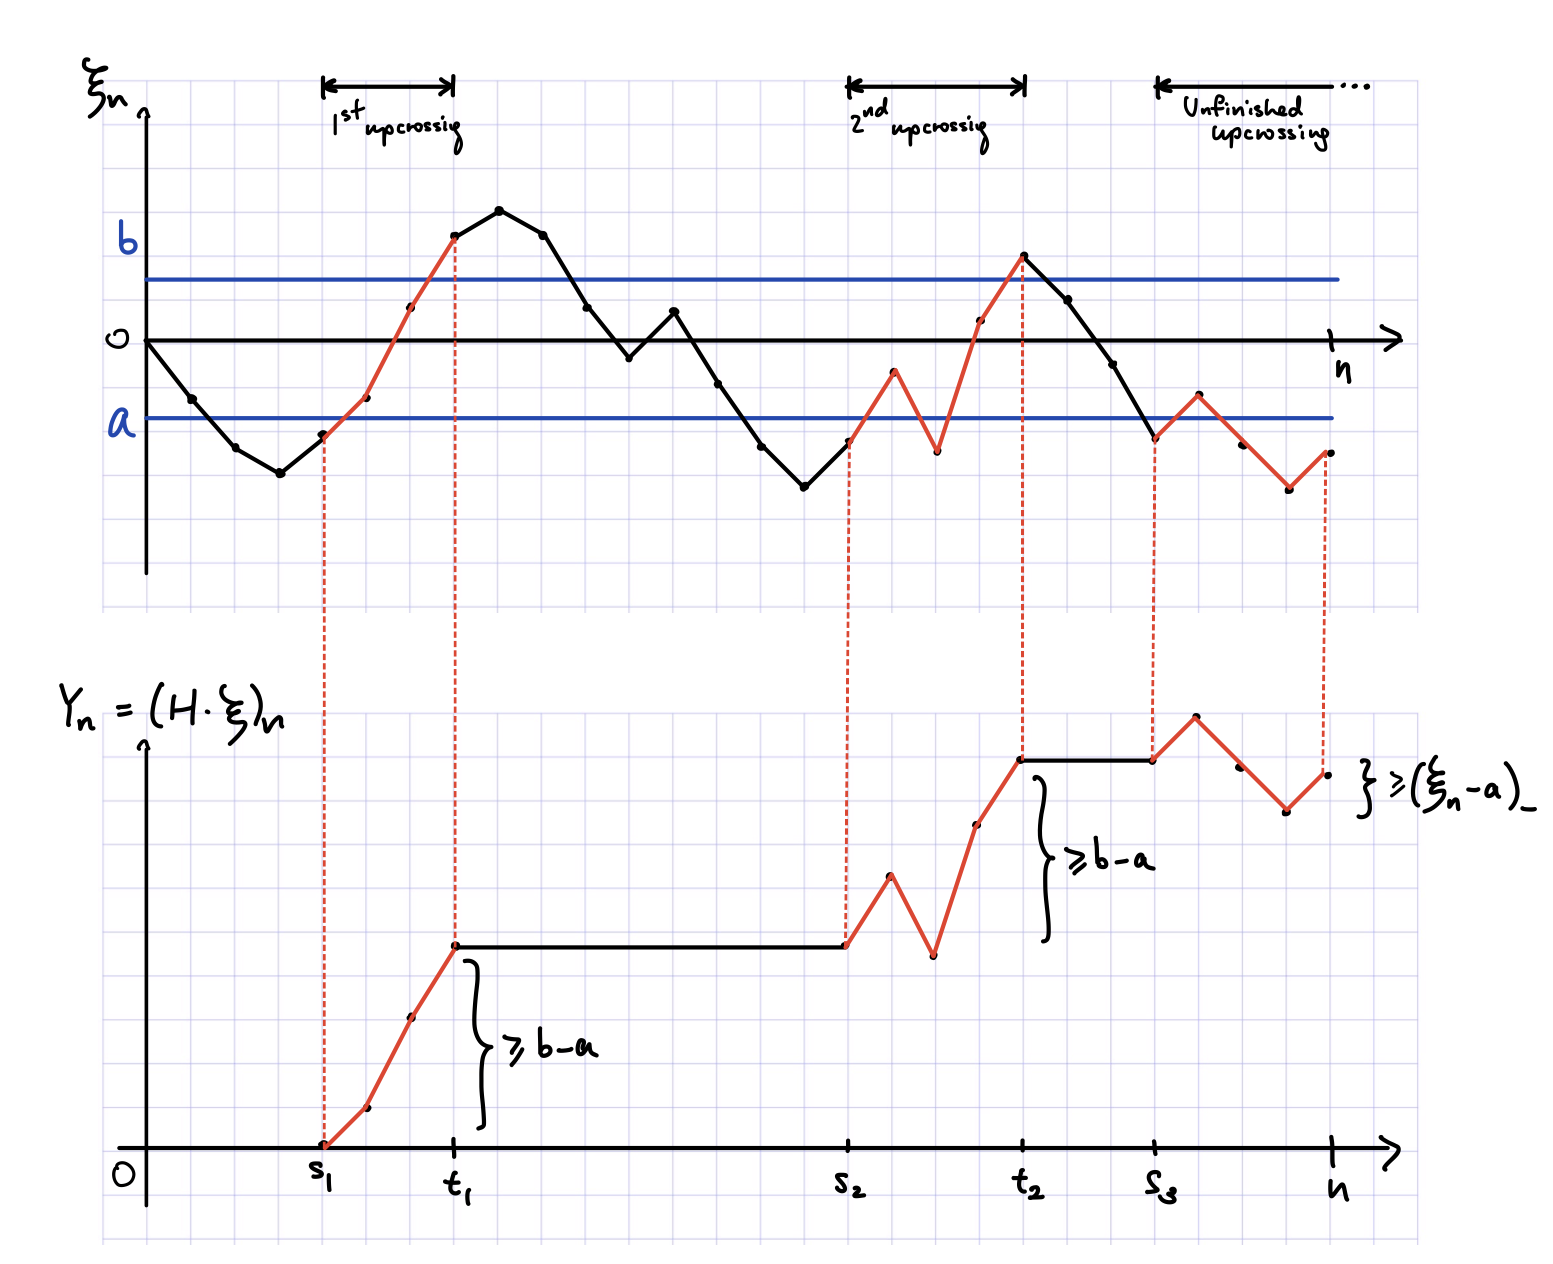
\includegraphics[width=\textwidth]{figures/upcrossing.png}
\captionof{figure}{An illustration of how we obtain $H\cdot \xi$ from $\xi$.}
\end{center}

The figure above shows an instance of $\xi$ with $U(\xi,[a,b],n)=2$, $Y = H\cdot \xi$ and how inequality \eqref{eq:decomposition_of_H_dot_X} is true. Taking expectation on both sides of \eqref{eq:decomposition_of_H_dot_X} and rearranging yields the upcrossing inequality.
\end{proof}

As a result, we have the following martingale convergence theorem.
\begin{theorem}[Almost sure (super-/sub-) martingale convergence theorem] \label{thm:as_mart_ct}
If $\xi = (\xi_n)_{n\geq 1}$ is a $\F_n$-adpted uniformly bounded super- (or sub-) martingale (with $\sup_n \E|\xi_n| = M < +\infty$) on $(\Omega,\F,\p)$, then $\xi_n$ converges $\p$-almost surely to some random variable $\xi_\infty \in L^1$.
\end{theorem}

\begin{proof}
Assume wlog that $\xi$ is a super-martingale. By upcrossing inequality (lemma \ref{lem:upcrossing_ineq}) we have, for all $n \geq 0$,
\begin{equation}
    \E\sqbracket{U(\xi,[a,b],n)} \leq \frac{\E(\xi_n - a)_-}{b-a} \leq \frac{\E\sqbracket{\abs{\xi_n}+\abs{a}}}{b-a} \leq \frac{M+\abs{a}}{b-a} < +\infty,
\end{equation}
therefore by Fatou's lemma,
\begin{equation}
    \E\sqbracket{U(\xi,[a,b])} \leq \frac{M+\abs{a}}{b-a} < +\infty.
\end{equation}
Therefore, given fixed $a,b \in \R$ we have $U(\xi,[a,b])<+\infty$ almost surely. Indeed, we may further conclude that for almost all $\omega$ we have $\forall a,b \in \Q, \; U(\xi,[a,b])<+\infty$. By lemma \ref{lem:relation_between_upcrossing_and_limit}, the following function is well-defined for $\p$-almost all $\omega$:
\begin{equation}
    \xi_\infty(\omega) = \lim_{n\to\infty} \xi_n(\omega) \in [-\infty,\infty].
\end{equation}
We may extend the function so that $\xi_\infty$ is well-defined on the entire $\Omega$. It remains to check that $\xi_\infty$ is in $L^1$, which follows from the Fatou's lemma directly that $\E[\abs{\xi_\infty}] \leq \liminf_{n\to\infty} \E[\xi_n] \leq M < +\infty$.
\end{proof}

\begin{exercise}
Show that if $(\xi_n)_{n\geq 0}$ is a sub-martingale with $\sup_{n} \E[(X_n)_+]$ then the above a.s. martingale CT still holds. Can you also weaken the a.s. martingale CT for super-martingales?
\end{exercise}

\begin{hint}
The main challenge is to check that the almost sure limit $\xi_\infty$ is in $L^1$.
\end{hint}

If we know further that $(\xi_n)$ is uniformly integrably, then we have the following stronger martingale CT for free
\begin{corollary}[Uniformly integrable super-/sub-martingale convergence theorem]
For a super-/sub-martingale $\xi=(\xi_n)_{n\geq 1}$, the following are equivalent:
\begin{enumerate}
    \item $(\xi_n)_{n\geq 1}$ is uniformly integrable,
    \item $(\xi_n)_{n\geq 1}$ converges almost surely and in $L^1$ to some $\xi_\infty \in L^1$
    \item $(\xi_n)_{n\geq 1}$ converges in $L^1$.
\end{enumerate}
\end{corollary}

\begin{proof}
$(1) \implies (2)$ is followed by the almost-sure martingale CT (theorem \ref{thm:as_mart_ct}) and the Vitali convergence theorem (theorem \ref{thm:vitali_convergence}). $(2) \implies (3)$ is trivial. $(3) \implies (1)$ is again a result of Vitali convergence theorem.
\end{proof}

As a reminder, the above result is not generally true. This could be seen in asymptotic random walks (special case 2 after example \ref{eg:product_of_indpt_rv}). Let us prove an even more surprising result for the case when $\xi$ is a martingale:
\begin{corollary}
If $\xi$ is indeed a martingale then $\xi_n = \E\sqbracket{\xi_\infty \,|\, \F_n}$.
\end{corollary}
\begin{proof}
This follows from the definition of conditional expectation, by choosing $A \in \F_n$ and showing that $\E\sqbracket{(\xi_n-\xi_\infty)\chi_A} \to 0$.
\end{proof}


\subsection{Application to proving 2nd OST}

\subsection{Random walk revisited}

\subsection{Galton-Watson Chain}

\subsection{Azuma-Hoeffding Inequality}

\subsection{Cadalag modification of continuous-time martingale}

% \subsection{Case study in optional pricing}

% \subsection{Further considerations for continuous-time martingale}